\section{Демонстрация работы кластера}

На листинге~\ref{config2} представлен конфиг кластера, который содержит 5 узлов, лидером будет являться \textit{node1}. Топология выбрана таким образом,
чтобы удовлетворяло "правилу большинства", которое заключается в том, чтобы кворум (количество узлов, принимающих участие в консенсусе) состоял не менее,
чем из $\lceil \frac{N}{2} \rceil + 1$. N -- общее количество узлов. Согласно этой формуле, кластер может гарантировать корректность работы
вплоть до момента, когда останется не менее 3 узлов.

\listing[
    caption={Пример конфигурационного файла для распределенного кластера},
    label=config2
]{assets/config.yml}

\subsection{Старт кластера}

На рисунке~\ref{fig:fig4} показан вывод команды \textit{start}, которая запускает все инстансы, указанные в конфиге, путь которого передана в аргументах
командной строки.

\begin{figure}
  \centering
  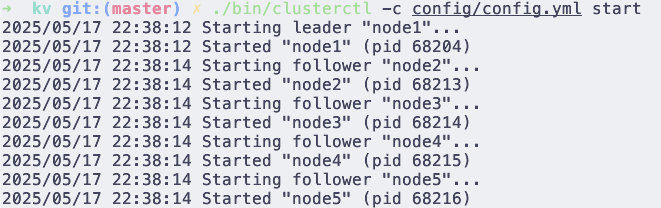
\includegraphics[scale=0.6]{assets/start.png}
  \caption{вывод комнды "clusterctl start"}
  \label{fig:fig4}
\end{figure}

На выводе представлен лог программы, где говорится о запуске каждого инстанса и ролью, которая соответствует ему. Также указан id процесса (pid) для
каждого узла хранилища.

Для того, чтобы узнать текущую топологию кластера, нужно воспользоваться командой \textit{status}. Пример вывода команды представлен на рисунке~\ref{fig:fig5}.

\begin{figure}
  \centering
  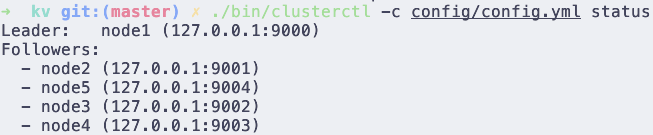
\includegraphics[scale=0.6]{assets/status.png}
  \caption{вывод комнды "clusterctl status"}
  \label{fig:fig5}
\end{figure}

На выводе виден список узлов и имя лидера с указанием адресов, которые указывают на RPC протокол.

Далее необходимо рассмотреть поведение узлов (как лидера, так и ведомого) в контексте протокола Raft при старте.
Для этого надо проанализировать их логи. На рисунке~\ref{fig:fig6}

\begin{figure}
  \centering
  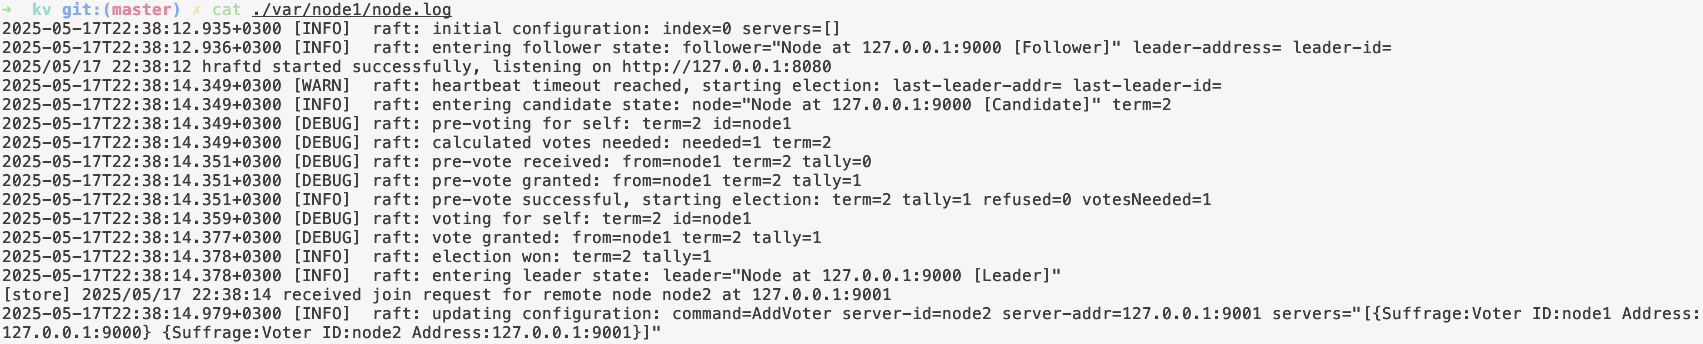
\includegraphics[scale=0.28]{assets/leader_logs.png}
  \caption{Логи лидера при старте}
  \label{fig:fig6}
\end{figure}

После инициализации конфигурации Raft узел входит в состояние "Follower", ожидая сигналов от лидера. Поскольку сигналов от лидера не поступает, узел переходит
в состояние "Candidate" и начинает процесс выборов, увеличивая термин. Он сначала проводит предварительное голосование для себя, затем, получив достаточное
количество голосов, запускает основное голосование. Узел выигрывает выборы и становится лидером кластера.

После этого лидер начинает принимать JOIN запросы на добавление новых узлов в кластер и обновляет конфигурацию, добавляя новые узлы, такие как \textit{node2},
\textit{node5}, \textit{node3} и \textit{node4}. На рисунке~\ref{fig:fig7} продемонстрированы логи лидера о вступлении новых узлов в консенсус.

\begin{figure}
  \centering
  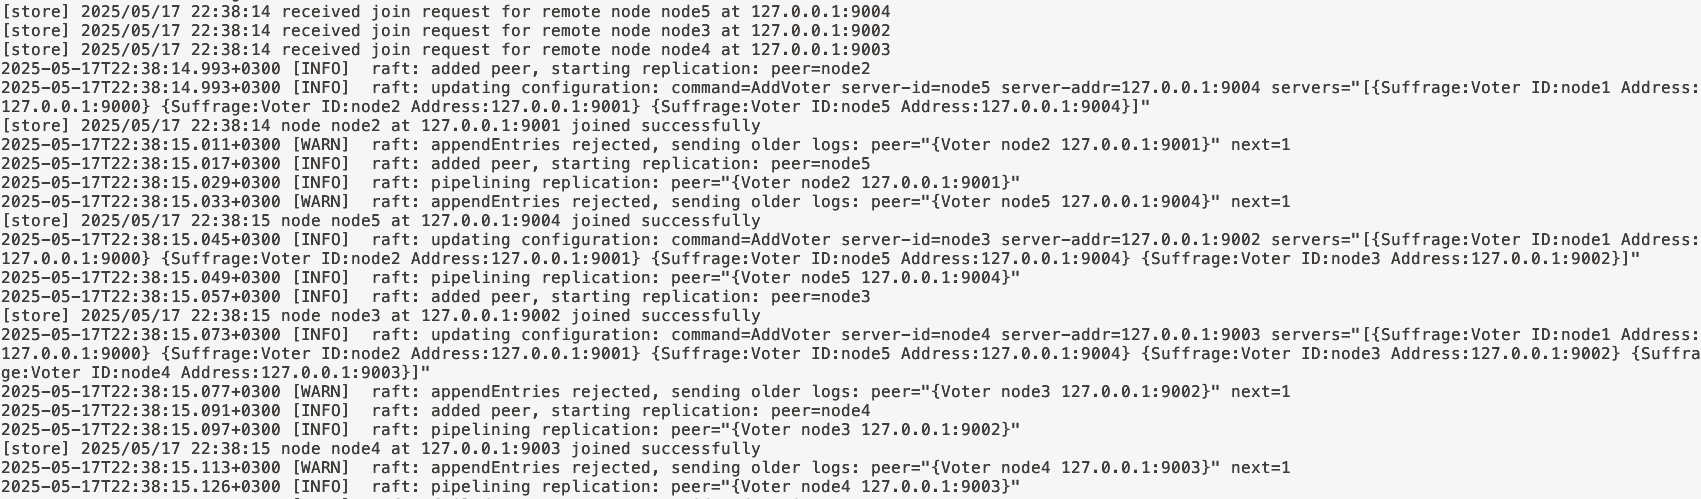
\includegraphics[scale=0.28]{assets/join_logs.png}
  \caption{Логи лидера при обработке JOIN запросов}
  \label{fig:fig7}
\end{figure}

Для каждого нового узла начинается процесс репликации данных с лидера, при этом для синхронизации отправляются старые записи в случае отклонения записей от узлов
с устаревшими данными. После успешного присоединения всех узлов кластер начинает работать с обновленной конфигурацией.

Со стороны "ведомых узлов" та же ситуация прсоединения к лидеру представлена на рисунке~\ref{fig:fig8}.

\begin{figure}
  \centering
  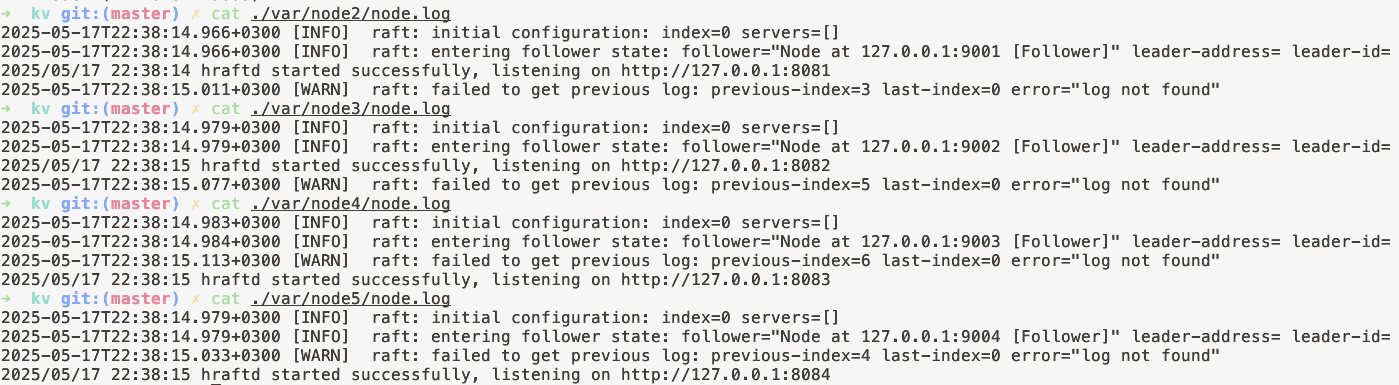
\includegraphics[scale=0.35]{assets/follower_join_logs.png}
  \caption{Логи ведомых узлов при присоединении к лидеру}
  \label{fig:fig8}
\end{figure}

\subsection{Операции с данными над кластером}

Для того, чтобы вставить данные на кластер, нужно отправить POST запрос на лидер-узел. Для того, чтобы прочитать данные с кластера, достаточно отправить GET
запрос с запрашиваемым ключом на любой узел. Отправка запроса представлена на рисунке~\ref{fig:fig7} при помощи утилиты curl.

\begin{figure}
  \centering
  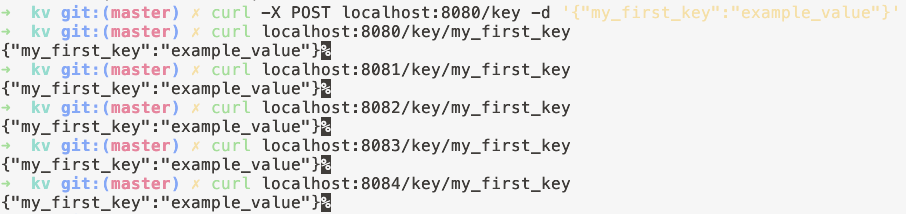
\includegraphics[scale=0.5]{assets/insert.png}
  \caption{Вставка данных на кластер}
  \label{fig:fig9}
\end{figure}

Данные, записанные на лидер, появились на остальных узлах, что говорит об успешной репликации.

Для того, чтобы удалить значение по ключу, необходимо отправить DELETE запрос на лидер-узел. Отправка запроса представлена на рисунке~\ref{fig:fig8}.

\begin{figure}
  \centering
  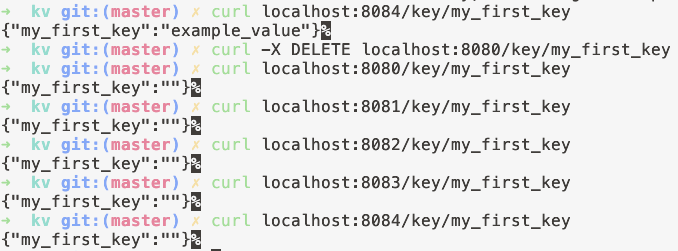
\includegraphics[scale=0.5]{assets/delete.png}
  \caption{Удаление данных с кластера}
  \label{fig:fig10}
\end{figure}

Чтение данных узлов показываются на предыдущих двух рисунках, чтобы проверить что данные вставились или удалились. Для этого необходимо отправить GET запрос
с ключом, значение которого нужно прочитать.

\subsection{Тестирование системы на отказоустойчивость}

Теперь, когда все возможности системы были показаны, необходимо проверить выполнение главного критерия, которым должна обладать система -- отказоустойчивость.

Перед проведением тестов необходимо заполнить хранилище различными значениями. Заполнение представлено на рисунке~\ref{fig:fig11}.

\begin{figure}
  \centering
  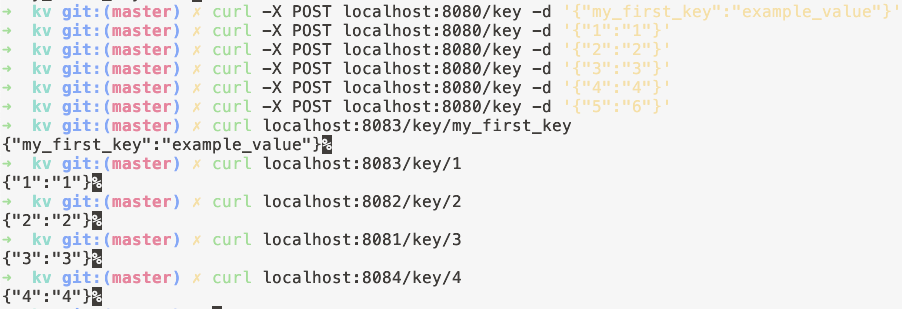
\includegraphics[scale=0.5]{assets/fill_in.png}
  \caption{Заполнение хранилища данными}
  \label{fig:fig11}
\end{figure}

Сейчас лидером является узел \textit{node1}. Далее необходимо сэмулировать сутуацию, применимую к реальной жизни, когда узел по какой-либо причине может отказать.
Например, возникли проблемы в сети, случился перебой в электричестве, процесс упал с ошибкой и т.д. Мы же просто отправим сигнал перывания на лидирующий узел.
Остановка лидера показана на рисунке~\ref{fig:fig12}.

\begin{figure}
  \centering
  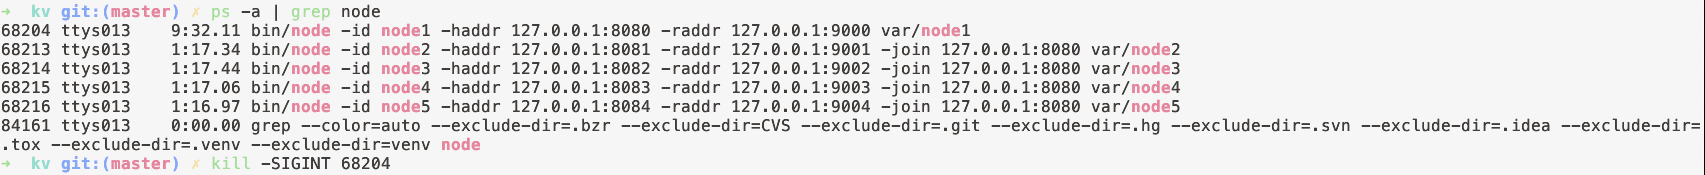
\includegraphics[scale=0.28]{assets/kill_leader.png}
  \caption{Остановка лидирующего узла}
  \label{fig:fig11}
\end{figure}

Как видно на рисунке, сначала был найден нужный PID узла-лидера, а затем на него был отправлен сигнал прерывания SIGINT.

Необходимо проверить, что случилось с кластером после падение лидера. Вызов команды status показан на рисунке~\ref{fig:fig12}.

\begin{figure}
  \centering
  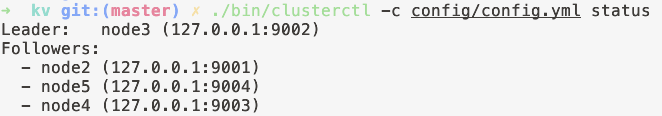
\includegraphics[scale=0.5]{assets/status_after_election.png}
  \caption{Статус кластера после выбора нового лидера}
  \label{fig:fig12}
\end{figure}

Узл \textit{node1} больше не показывается, так как он был остановлен. Теперь лидером является \textit{node3}. Нужно убедиться, каким образом был выбран третий
узел. Для этого нужно взгялнуть на логи узлов для детального разбора этапа голосования.

На рисунке~\ref{fig:fig13} представлены логи выбора нового лидера -- \textit{node3}.

\begin{figure}
  \centering
  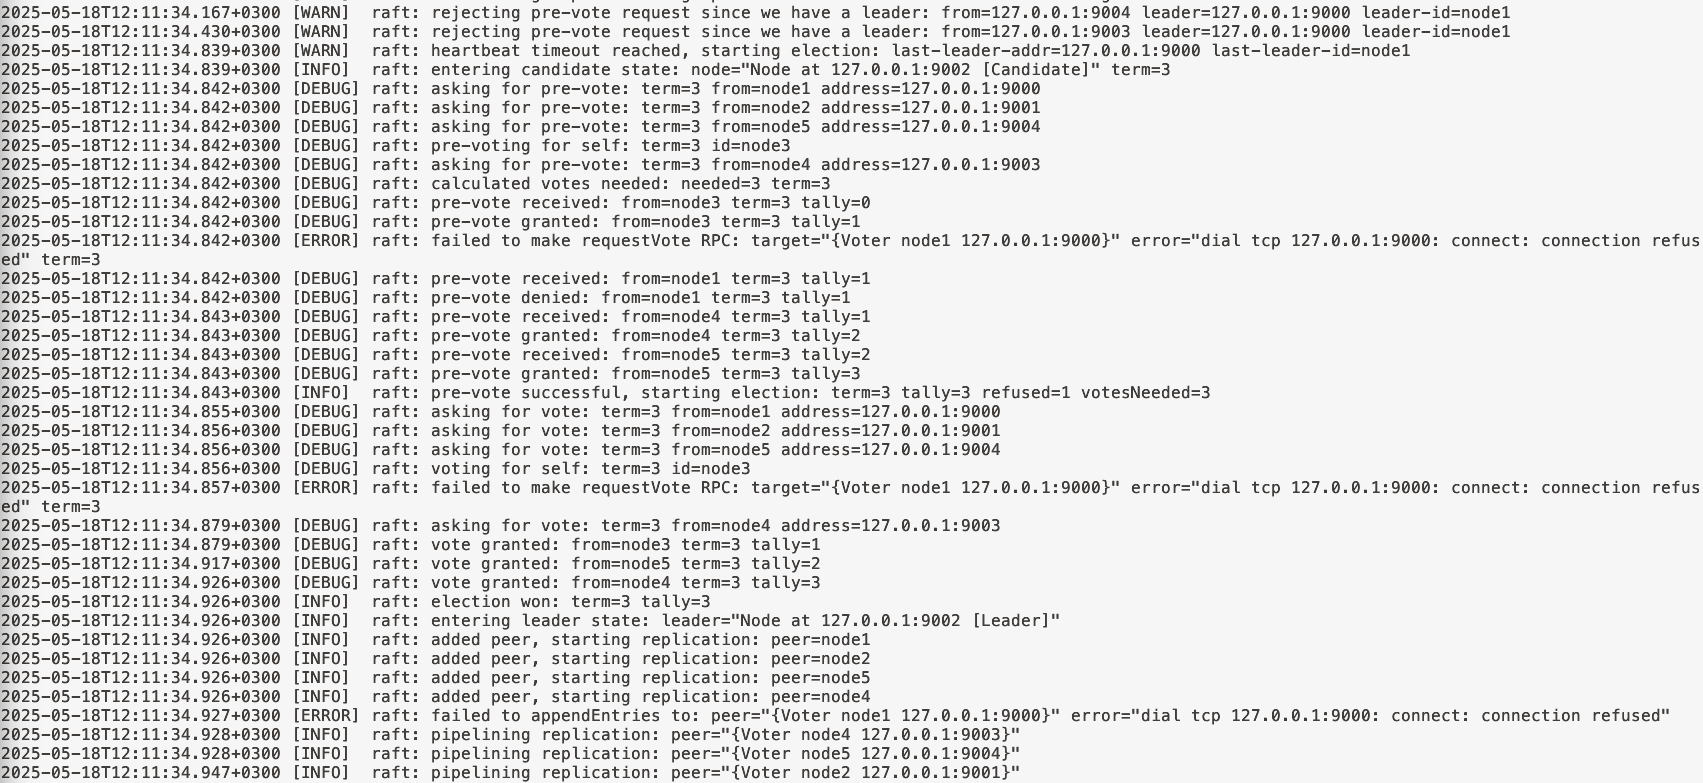
\includegraphics[scale=0.28]{assets/new_leader_election.png}
  \caption{Процесс выбора нового лидера}
  \label{fig:fig13}
\end{figure}

После того как предыдущий лидер (Узел 1) был остановлен, узлы начали процесс выборов, и Узел 3 перешёл в состояние "Candidate". Он начал запрашивать голоса у
других узлов и получал предварительные голоса, включая поддержку от Узла 5. Получив достаточное количество голосов, Узел 3 продолжил выборы, голосуя за себя и
получая окончательные голоса. В результате, Узел 3 выиграл выборы, стал лидером и перешёл в состояние "Leader". После этого он начал принимать новые узлы в
кластер, включая Узлы 1, 2 и 4, и инициировал репликацию данных для синхронизации всех узлов. В конечном итоге все узлы были успешно синхронизированы, и Узел 3 продолжил оставаться лидером кластера.

Для ведомых узлов представлен процесс голосования на примере \textit{node4}. Его логи представлены на рисунке~\ref{fig:fig14}.

\begin{figure}
  \centering
  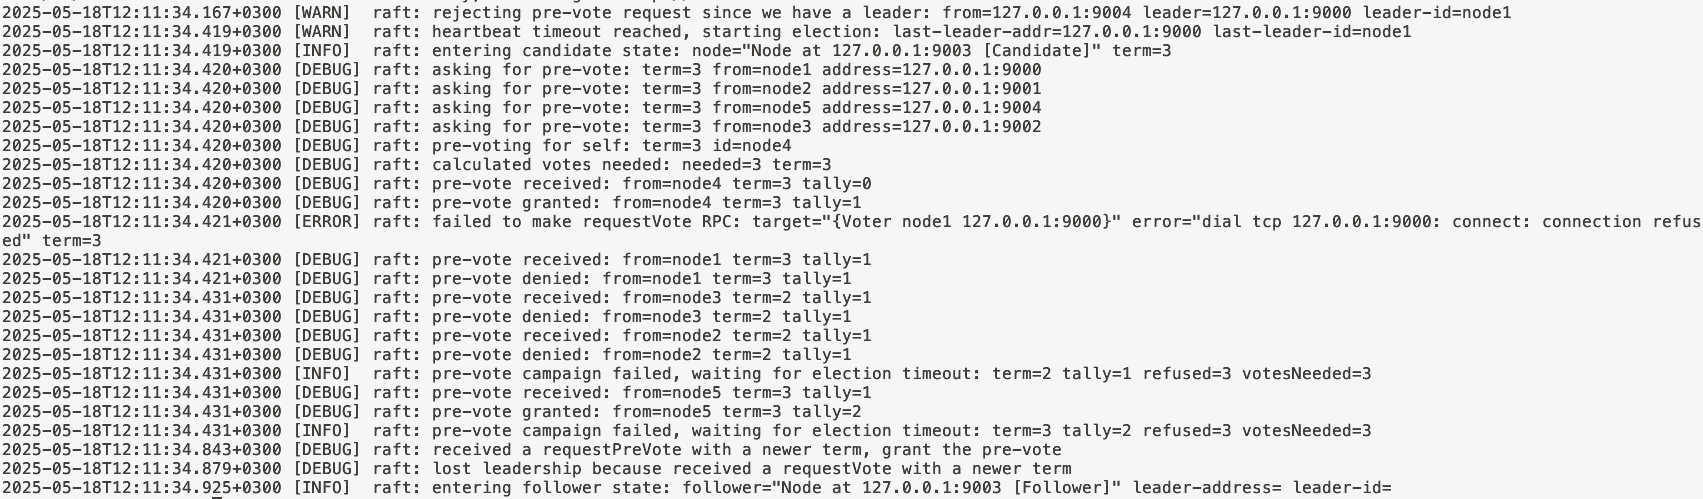
\includegraphics[scale=0.28]{assets/follower_election.png}
  \caption{Процесс выбора нового лидера со стороны ведомого узла}
  \label{fig:fig14}
\end{figure}

Когда Узел 3 начал процесс выборов, Узел 1, оставшийся в прежнем статусе, отклонил предварительные запросы на голосование, поскольку у него уже был лидер.
Узел 2 и другие узлы начали свои выборы, переходя в состояние "Candidate", и начали собирать голоса, но узел 2 столкнулся с ошибкой подключения при попытке
голосовать с Узлом 1, так как тот больше не мог участвовать в голосовании. Узел 2 продолжал пытаться собрать голоса, но не смог набрать достаточное количество,
поскольку другие узлы также не поддержали его. В итоге Узел 2 и другие узлы вернулись в состояние "Follower", ожидая нового лидера, которым стал Узел 3.

Необходимо проверить, что после выбора нового лидера данные остались. На рисунке~\ref{fig:fig15} представлена работа с данными.

\begin{figure}
  \centering
  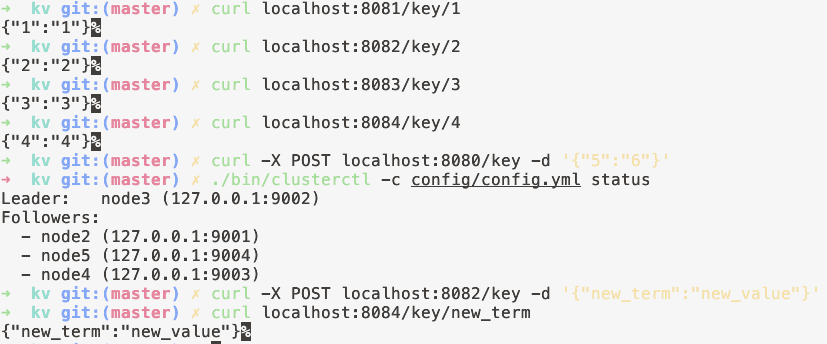
\includegraphics[scale=0.5]{assets/new_term_crud.png}
  \caption{Работа с данными в новом терме}
  \label{fig:fig15}
\end{figure}

Как видно на рисунке, представленном выше, данные не потерялись. После вставки нового ключа на нового лидера, данные успешно реплецировались на все его реплики.
Таким образом был достигнут и проверен консенсус между узлами кластера с помощью алгоритма Raft.

После тестов необходимо остановить кластер. Остановка кластера продемонстрирована на рисунке~\ref{fig:fig15}.

\begin{figure}
  \centering
  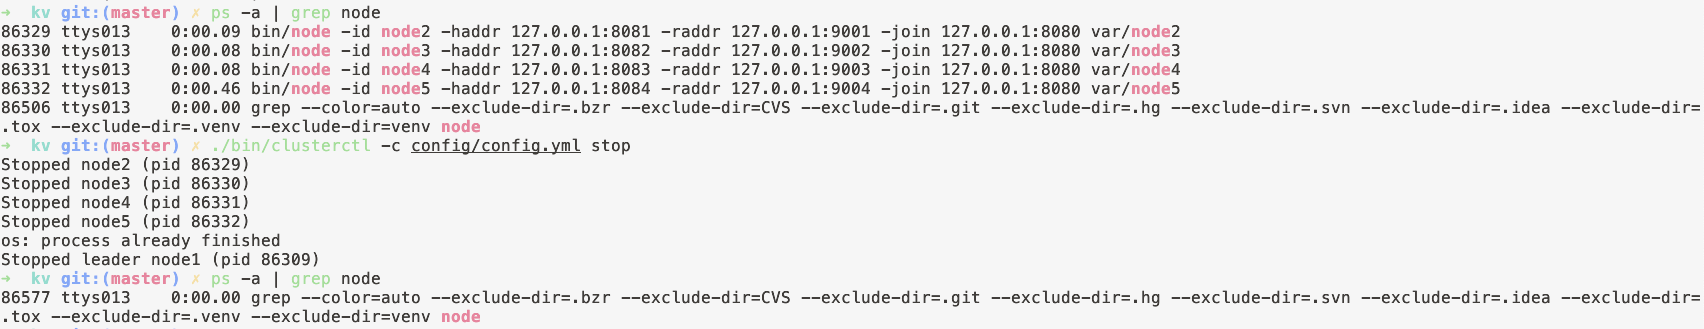
\includegraphics[scale=0.28]{assets/stop.png}
  \caption{Остановка всего кластера}
  \label{fig:fig15}
\end{figure}

На рисунке выше показан вывод всех живых узлов до остановки, вызов команды stop, а затем проверка того, что все процессы исчезли, что свидетельствует о корректной
работе команды.
